%!TEX root = ../../super_main.tex

\subsection{Temporal Properties of Snapshots}
\label{sec:temporal_properties_of_snapshots}

% We go under the assumption that it will be possible to eaves drop in at all times meaning that we can retrieve a measurement from any sensor at all times, however this is not the case but this assumption is maintained as described in \secref{sec:providing_sensor_data}. We have structured the data from the sensors, with the assumption of the sensor availability, to be collected as shown in \figref{fig:sample_temporality}. In this figure we see \emph{measurement} instances which each correspond to one reading or value of a sensor in a snapshot. 
% \\\\

\todo[inline]{Den her subsection skal have en god introduktion, men for lidt hjerne betyder at vi ikke kan lave den lige nu.}

We introduce a collection of such measurements which we call a \emph{sample}, because a single \emph{measurement} from a continuous sensor often does not make much sense on its own. A single measurement from an accelerometer, for instance, does not describe the context in which the participants exists well as a few consecutive measurements from where a tendency can be derived, i.e. whether a participant's acceleration is constant in the same direction or whether the acceleration is slowing down.
\\\\
A \emph{sample} is thus simply a stream of \emph{measurement} instances where the interval or frequency (\emph{measurement frequency}) between them is configurable as seen in \figref{fig:sample_temporality}. Furthermore, we want customers to configure how often these \emph{sample}s should be gathered, and for that reason we allow them to define a \emph{sample frequency}. And lastly the length of the of the snapshots is configurable by defining a \emph{total duration}, which states for how long samples should be generated for a snapshot.

\begin{figure}[!htbp]
    \centering
    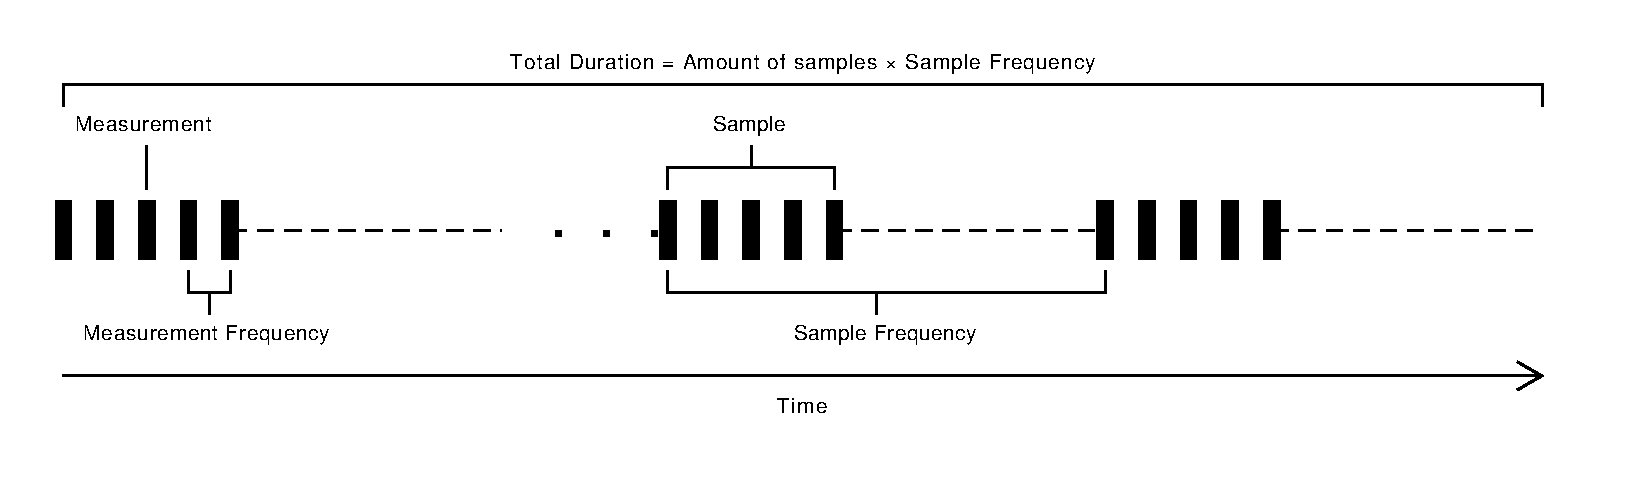
\includegraphics[width=\textwidth]{gathering_sensor_data/sample_temporality}
    \caption{Illustration of temporality for samples for a single sensor in a snapshot.}
    \label{fig:sample_temporality}
\end{figure}
\FloatBarrier

By this temporal structure of the sensor data we provide a viable way of configuring how the snapshots should be structured in regards to sensor readings, while maintaining a uniform output format for customers of the system.
